%% \chapter{Introduction \Author{J. Singer}\\\progressbar[0.4\textwidth]{draft}{70}}
\chapter{Introduction \Author{J. Singer}}


%%%%%%%%%%%

% Possibility of unique names for distinct entities.
% Maybe a slightly humorous example, involving Homer Simpson and
% Homer the classical Greek poet. Convey the point that,
% without unique names, extra \textit{context} is required
% to make the name useful.
% (Springfield or Greece?)

In computer programming, as in real life, 
names are useful handles for concrete entities.
% Discuss the utility of names as abstract identifiers.
The key message of this book is that
having \textit{unique names} for
\textit{distinct entities}
reduces uncertainty and imprecision.

For example, consider overhearing a conversation
about `Homer.' Without any more contextual clues, you
cannot disambiguate between Homer Simpson and Homer the
classical Greek poet; or indeed, any other people
called Homer that you may know.
As soon as the conversation mentions Springfield
(rather than Smyrna), you are fairly sure that the
Simpsons television series (rather than Greek poetry)
is the subject.
On the other hand, if everyone had a \textit{unique} name,
then there would be no possibility of confusing 20th century
American cartoon characters with ancient Greek literary figures.
\textit{Could we have a cartoon picture here?}

% where SSA is applied, in compiler intermediate representations...
This book is about the \textit{static single assignment form} (SSA),
which is a naming convention for storage locations (variables)
in low-level representations
of computer programs.
%% remove following definition, since we have a full Section
%% on definition coming up soon...
% A program is said to be in SSA form when each variable is defined (hence
% \textit{assignment})
% exactly once (hence \textit{single}) in the program text
% (hence \textit{static}).
The term \textit{static} indicates that SSA is particularly
relevant for program analysis that occurs inside a 
compiler, prior to execution.
The term \textit{single} refers to the uniqueness property of
variable names that SSA imposes. As illustrated above, this enables
more accurate analysis.
The term \textit{assignment} means variable definitions. For
instance, in the code 
\begin{verbatim}
x := y+1
\end{verbatim}
the variable $x$ is being assigned the value of expression $(y+1)$.
This is a definition, or assignment, of $x$.

%%%%%%%%%%%%%%%%%%%%%

\section{Definition of SSA}


The seminal paper on SSA 
\cite{cytron91efficiently}
gives an informal prose
definition as follows:

\begin{quotation}
A program is defined to be in SSA
form if each variable is a target of
exactly one assignment statement in the
program text.
\end{quotation}

% Informally, static means `program text.'
% single means `unique names'
% assignment means `at variable definitions.'

%% Again, informally, unique definition for each variable.

This is the simplest,
least constrained, definition of SSA. However
there are various, more specialized, varieties of SSA,
which impose further constraints on programs.
Such constraints are generally expressed in terms
of dominance properties of variable definitions, or
the presence or absence of certain 
pseudo-functions at control-flow merge points.
% Formally, in terms of dominance. Each var has a unique
% definition, and def dominates all uses.
% Perhaps require implicit defs of all vars at entry,
% implicit uses of all vars at exit?
Each distinct SSA flavour has specific characteristics---many of
these are discussed in Chapter \ref{FIXME} 2.
% forward links to Philip's discussion of
% SSA flavours and properties here

One important property that holds for all forms of SSA,
including the simple definition above, is 
\emph{referential transparency}.
Since there is only a single definition for each variable
in the program text, a variable's value
is \textit{independent of
its position} in the program.
(We may refine our knowledge about a particular variable
based on branching conditions, e.g.\ we know the value of $x$ in the
\texttt{then} branch following a \texttt{if (x==0)} statement; however the
\textit{underlying value} of $x$
does not change at this \texttt{if} statement.)
Programs written in pure functional languages
are referentially transparent.

Referentially transparent programs are more amenable to 
formal methods and mathematical reasoning, since
the meaning of an expression depends only on the
meaning of its subexpressions
and not on the order of evaluation or
side-effects of other expressions.

For a referentially opaque program, consider
the following code fragment.
\begin{verbatim}
x := 1;
y := x + 1;
x := 2;
z := x + 1;
\end{verbatim}
A naive (and incorrect) analysis may assume that the values
of $y$ and $z$ are equivalent, since they have identical 
assignments of $(x+1)$. 
However the value of variable $x$ depends on whether
the current code position is before or after the second assignment
to $x$, i.e.\ variable values depend on their \textit{context}.

When a compiler transforms this program fragment to SSA code,
it becomes referentially transparent. The translation process
involves renaming to  
eliminate multiple assignments to the same variable. Now it is
apparent that $y$ and $z$ are only equivalent if $x1$ and $x2$
are equivalent.
\begin{verbatim}
x1 := 1;
y  := x1 + 1;
x2 := 2;
z  := x2 + 1;
\end{verbatim}


% "The most important feature of mathematical notation is that an expression is used solely to describe (or denote) a value. In other words, the meaning of an expression is its value and there are no other effects, hidden or otherwise, in any procedure for actually obtaining it. Furthermore, the value of an expression depends only on the values of its constituent expressions (if any) and these subexpressions may be replaced freely by others possessing the same value. ... The characteristic property of mathematical expressions described here is called "referential transparency." Bird, Richard, and Wadler, Philip; Introduction to Functional Programming, p. 4; Prentice Hall, 1988.


%%%%%%%%%%%%%%%%%%%%%



\section{Informal Semantics of SSA}

% including examples


In the previous section, we saw how straightline sequences of code
can be transformed to SSA by simple renaming of variable definitions.
The \textit{target} of the definition is the variable being defined, on the
left-hand side of the assignment statement.
In SSA, each definition target must be a unique variable name.
On the other hand, variable names can be used multiple times
on the right-hand side of any assignment statements, as 
\textit{source} variables for definitions.
Throughout this book, renaming is generally performed by 
adding integer subscripts to original variable names;
however in general this is an unimportant implementation feature.

% Given a simple pseudo-code language, show examples of programs in SSA.
% (Should I show before/after SSA transformation, or just programs
% in SSA form already? Fabrice suggests before/after... plus
% one or two sentences commentary on each.)

The \textit{$\phi$-function} is the most important SSA concept to grasp.
%% (Explain carefully how $\phi$-functions work.) 
It is a special statement, known as a
\textit{pseudo-assignment} function.
Appel \cite{appel97modern} calls it a `notational fiction.'
\footnote{
% Date: Wed, 16 Jun 2010 17:23:00 -0400
% From: Kenneth Zadeck <zadeck@naturalbridge.com>
% To: Jeremy Singer <jsinger@cs.man.ac.uk>
% Subject: Re: SSA book
% References: <4C18E277.4090605@cs.man.ac.uk>
% In-Reply-To: <4C18E277.4090605@cs.man.ac.uk>
%
% i would add that this was something of an inside joke.  But it did serve
% as the basis for the name that we ended up using.   
%
% On 06/16/2010 10:40 AM, Jeremy Singer wrote:
% > Hi Kenny,
% > Hope you are well. I am writing an introductory chapter for the SSA
% > textbook that was proposed at the SSA seminar in France last year. When
% > I introduce phi-functions, I want to put a footnote that says something
% > like:
% >
% > Kenneth Zadeck reports that $\phi$-functions were originally known
% > in-house as \textit{phoney}-functions, during the development of SSA at
% > IBM Research.
% >
% > Is this a fair comment? Would you like me to change it at all?
% >
% > Thanks for your help.
% > Best regards,
% > Jeremy
% >
% > ---
% > http://www.cs.man.ac.uk/~jsinger
% >
Kenneth Zadeck reports that $\phi$-functions were originally
known as \textit{phoney}-functions, during the development
of SSA at IBM Research. Although this was an in-house joke,
it did serve as the basis for the eventual name.
}
The purpose of a $\phi$-function is to merge
values from different incoming paths, at control-flow
merge points.

Consider the following example:

\begin{verbatim}
x := input();
if (x == 42)
    y := 1;
else
    y := x*2;
print(y);
\end{verbatim}

There is a distinct definition of $y$ in each branch of the \texttt{if}
statement. So multiple definitions of $y$ reach the \texttt{print} statement
at the control-flow merge point. When a compiler transforms this program 
to SSA,
the multiple definitions of $y$ are renamed as $y1$ and $y2$. However 
the \texttt{print} statement could use either variable, dependent on the
outcome of the \texttt{if} conditional test. A $\phi$-function introduces
a new variable $y3$, which takes the value of either $y1$ or $y2$.
Thus the SSA version of the program is:

\begin{verbatim}
x := input();
if (x == 42)
    y1 := 1;
else
    y2 := x*2;
y3 := \phi(y1,y2);
print(y3);
\end{verbatim}



At the start of a block of code, the $\phi$-function has
$n$ parameters if there are $n$ incoming control-flow paths to this block.
The behaviour of the $\phi$-function is to select the value
of the parameter associated with the actually executed control-flow path.
This value is assigned to the fresh variable name, on the left-hand-side
of the $\phi$-function.
Such pseudo-functions are required to maintain the SSA property
of unique variable definitions,
in the presence of non-sequential control flow.

\textit{FIXME - I'm worried about the order of information
presented in these paragraphs. I think it all needs to be there,
but maybe it could be organized more intuitively... -jsinger}

It is important to note that, if there are multiple $\phi$-functions
at the head of a basic block, then these are executed simultaneously,
\textit{not} sequentially.
This distinction becomes important if the target of a $\phi$-function
is the same as the source of another $\phi$-function, perhaps after
optimizations such as copy propagation. \textit{(ref later chapters?)}
When $\phi$-functions are eliminated in the SSA destruction phase,
they are replaced by parallel copy operations.
% at the end of predecessor control flow nodes.
(forward note to Fabrice's section on this,
in later chapter).

Strictly speaking, $\phi$-functions are not directly executable,
since the dynamic control-flow path leading to the $\phi$-function
is not explicitly encoded as an input to $\phi$-function.
This is tolerable, since $\phi$-functions are only 
used during static analysis of the program. They are removed
before any program interpretation or execution takes place.
There are various executable extensions of $\phi$-functions, 
such as $\gamma$-functions, which take
an extra parameter to specify which source value to assign to the
target variable. (forward ref to VSDG chapter?)

\textit{FIXME - I would like an example of how to transform a 
while loop into SSA, showing how the $\phi$-function
must be placed at the loop header. Fabrice doesn't think this
example is necessary, but it would be helpful for beginners, I feel...
-jsinger}

%% loop illustrates difference between static and dynamic single/multiple
%% assignments -cck

example 3. while loop? (iteration)

\begin{verbatim}
x = 0;
y = 0;
while (x< 10) {
  y = y + x;
  x++;
}
print(y)
\end{verbatim}



%%%%%%%%%%%


%%%%%%%%%%%

\section{Comparison with Classical Data Flow Analysis}

% Very simple. Discuss lattice-based data flow analysis.
% Propagating facts around control-flow points in a CFG.

Data flow analysis collects information about programs
in order to make optimizing code transformations.
During actual program execution, information flows between
variables. Static analysis captures
this behaviour by propagating \textit{abstract} information,
or data flow facts,
using an operational representation of the 
program such as the CFG. This is the approach used in 
classical data flow analysis.

Often, data flow information can be propagated more efficiently
using a \textit{functional}, or \textit{sparse},
representation of the program such 
as SSA.
% Information that are only related to values can be efficiently 
% propagated using a more functional representation of the program
% along a more sparse evaluation graph (such as SSA).
When a program is translated into SSA form,
variables are renamed at definition points.
For certain data flow problems (e.g.\ constant propagation)
this is exactly the set of program points where data flow
facts may change.
Thus it is possible to associate data flow facts directly with 
variable names, rather than
maintaining a vector of data flow facts, indexed over all variables
at each program point.
% Talk about SSA simplification - rename whenever data flow
% facts can change (for a certain class of data flow problems?)
% Plain SSA - rename at variable definitions - so any data flow
% analysis where data flow properties change only with definitions
% (e.g. constant propagation) OK. 
For other data flow problems, properties may 
change at points that are not variable definitions.
These problems can be accommodated in a sparse analysis framework
by inserting additional pseudo-definition functions at appropriate 
points
to induce additional variable renaming. \emph{FIXME - forward pointers to
appropriate chapters?}


% Variables carry values.
% Analysis compute diverse information about those values.
% For engineering purposes, it is good to have one
% name/variable per different value and to store
% the value/information on the variable.
% A not very efficient alternative is to store the information
% for each couple (prog.point, variable) e.g. data flow analysis
% on the CFG.
% When the computed info depends only on variable definitions this
% leads to have one variable per def i.e. SSA.

The rest of this section presents a trivial example
data flow analysis: 
\textbf{non-zero value analysis}. 
For each variable in a program, the aim is to determine statically whether
that variable can contain a zero integer value at runtime.
Figure \ref{fig:part1-vanilla-nonzerolattice} shows the lattice of 
data flow facts. The analysis will assign an abstract value from this lattice
to each variable at each point in the program text.

\begin{figure}
\begin{center}
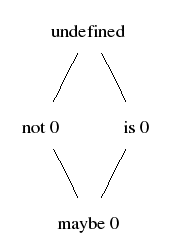
\includegraphics[scale=0.6]{zero_lattice.png}
\end{center}
\caption{\label{fig:part1-vanilla-nonzerolattice}Lattice of data flow facts
  for non-zero value analysis}
\end{figure}

Figure \ref{fig:part1-vanilla-cfgexample}(a) shows an example program CFG.
The full control flow structure of the program is given, however
it only shows definition
statements relating to variable $x$.
Figure \ref{fig:part1-vanilla-cfgexample}(b) shows the SSA version of this
example program. Full details of the SSA construction algorithm are given in 
Chapter \emph{FIXME - 3}. For now, it is sufficient to see that:
\begin{enumerate}
\item Integer subscripts have been used to rename
variable $x$ from the original program.
\item We have assumed an implicit definition of $x_0$ at the entry point of
  the program.
\item A $\phi$-function has been
inserted at the appropriate control-flow merge point where multiple reaching
definitions of $x$ converged in the original program.
\end{enumerate}


\begin{figure}
\begin{center}
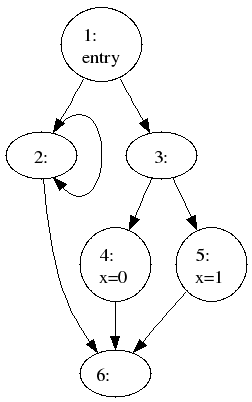
\includegraphics[scale=0.3]{cfg_example.png}
%
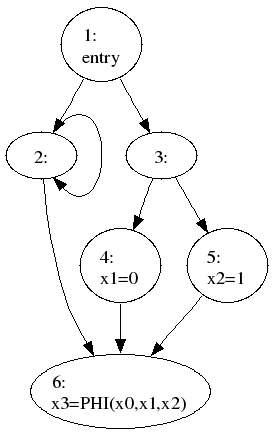
\includegraphics[scale=0.3]{ssa_example.png}
\end{center}
\caption{\label{fig:part1-vanilla-cfgexample}Example control flow graph for
  non-zero value analysis, only showing relevant definition statements for
  variable x, in both (a) non-SSA and (b) SSA form.}
\end{figure}


With classical data flow analysis on the CFG in Figure
\ref{fig:part1-vanilla-cfgexample}(a),
we would compute information about variable $x$ for each of the six nodes
in the CFG, using suitable data flow equations.
This might give results such as those shown in Table
\ref{tab:part1-vanilla-cfgres}.

\begin{table}
\begin{center}
\begin{tabular}{l|l} \hline
CFG node & abstract value of $x$ \\ \hline
1 & undefined \\
2 & undefined \\
3 & undefined \\
4 & is 0 \\
5 & not 0 \\
6 & maybe 0 \\ \hline
\end{tabular}
\end{center}
\caption{\label{tab:part1-vanilla-cfgres}Results of the CFG data flow analysis}
\end{table}

Using SSA-based data flow analysis on Figure 
\ref{fig:part1-vanilla-cfgexample}(b),
we compute information about each variable based on a simple
analysis of its definition statement. This gives us four data flow facts,
one for each SSA version of variable $x$, as shown in Table
\ref{tab:part1-vanilla-ssares}.

\begin{table}
\begin{center}
\begin{tabular}{l|l} \hline
SSA variable & abstract value \\ \hline
$x_0$ & undefined \\
$x_1$ & is 0 \\
$x_2$ & not 0 \\
$x_3$ & maybe 0 \\ \hline
\end{tabular}
\end{center}
\caption{\label{tab:part1-vanilla-ssares}Results of the SSA data flow
  analysis}
\end{table}


This illustrates several key advantages of the SSA-based analysis.
First, data flow
\textit{information propagates directly}
from definition statements to uses, via
the def-use links implicit in the SSA naming scheme. 
In contrast, the 
classical data flow framework 
propagates information throughout the program,
including points such as node 2 where the information 
about $x$ does not change, or is not relevant.
Second, the results of the SSA data flow analysis are
\textit{more succinct}.
There are four data flow facts (one for each SSA version of $x$)
versus six facts for the non-SSA program (one fact about variable $x$
per CFG node).

Part II 
\emph{FIXME - forward ref}
of this book gives a more comprehensive treatment of 
SSA-based data flow analysis.


%%%%%%%%%%%%%%%%

\section{SSA in Context}


% Crib most of this from Kenneth Zadeck. 

% Talk about other program dependence graph
% representations, 

\subsection{Historical Context}

Throughout the 1980s, as optimizing compiler
techology became more mature, various intermediate
representations (IRs) were proposed to encapsulate data
dependence in a way that enabled fast and accurate
data flow analysis.
The motivation behind the design of
such IRs was the exposure of direct links between variable
definitions and uses, known as \textit{def-use chains},
enabling efficient propagation of data-flow information.
% This gives the ability
% to propagate data flow information directly
% from definitions to uses,
% and vice versa.
Example IRs include the program dependence graph \cite{ferrante87program}
and program dependence web \cite{ottenstein90program}.
Chapter \ref{vsdg} VSDG? gives further details on dependence graph
style IRs.

% Talk about early developments at IBM in 1980s.
% Talk about eventual emergence of SSA.

Static single assignment form was one such IR, 
which was developed at IBM Research, and publicly announced
in several research papers in the late 1980s
\cite{rosen88global,alpern88detecting,cytron89efficient}.
SSA rapidly gained popularity due to its 
intuitive nature and straightforward
construction algorithm.
The SSA property gives a 
standardized shape for variable def-use chains,
which can simplify data flow analysis techniques.

\subsection{Current Usage}

The majority of current commercial and open-source compilers
use SSA as a key intermediate representation for
program analysis.
SSA is generally enabled with the \texttt{-O}
flag in ahead-of-time compilers (since SSA construction
is fairly expensive, and only required for optimization).
Similarly for just-in-time compilers, only the \textit{hot} 
methods will be recompiled with SSA-based optimizations.

All modern optimizing compiler infrastructures, e.g.\ LLVM, 
use SSA from the ground up.
Other compilers, e.g.\ GCC, began
development before SSA was well-characterized or
widely known.
In such cases, SSA support can be backported into 
the original optimization infrastructure.
For instance, GCC uses SSA as of version 4.0
\cite{novillo03tree,novillo04design}.
\textit{perhaps give forward pointer to Diego's chapter on the advantages
of SSA in gcc?}

\subsection{SSA for High-Level Languages}

So far, we have presented SSA as a useful feature for 
compiler-based analysis of low-level programs.
It is interesting to note that some high-level languages enforce
the SSA property.
The SISAL language is defined in such a way that
programs automatically have referential transparency, since
multiple assignments are not permitted to variables.
Other languages allow the SSA property to be
applied on a per-variable basis, using facilities like
Java \texttt{final} variables
and C\# \texttt{const} and \texttt{readonly} modifiers. 

The motivation for allowing the programmer to enforce
SSA in an explicit manner in high-level programs is that
\textit{immutability simplifies concurrent programming}.
Read-only data can be shared freely between multiple threads,
without any data dependence problems.
This is becoming an increasingly important issue, with the
trend of multi- and many-core processors.

High-level functional languages claim
referential transparency as one of the
cornerstones of their programming paradigm.
Thus functional programming supports the SSA property
implicitly.
Chapter \ref{} \textit{intro-semantics} details the 
dualities between SSA and functional programming.

% However in general,
% it is straightforward to translate a non-SSA program into an SSA
% program. (Links to appropriate chapters here?
% Simple construction / Advanced construction chapters.)



%%%%%%%%%%%%%%%%

\section{Benefits of SSA}

In this chapter, we have introduced the notion of SSA.
We now conclude by enumerating some of the benefits 
that it provides.

SSA imposes a strict discipline on variable naming in programs,
so that each variable has a unique definition point.
New names are introduced at variable assignments, and at control-flow
merge points.
This serves to simplify variable def-use relationships,
which underpin data flow analysis.
There are three main advantages that SSA enables:
\begin{description}
\item[Program runtime benefit]
Certain compiler optimizations can be more effective
when operating on programs in SSA form. These include the
class of \textit{control-flow insensitive analyses}.
\item[Compile time benefit]
Certain compiler optimizations can be more efficient
when operating on SSA programs, since
referential transparency means that data flow information
can be associated directly with variables, rather than with variables
at each program point.
\item[Compiler development benefit]
Program analyses and transformations can be easier
to express in SSA. This means that compiler engineers
can be more productive, in writing new compiler passes,
and debugging existing passes.
\texttt{FIXME - Any anecdotal experience from GCC - ask Diego?}
\end{description}



%%%%%%%%%%%
